\documentclass{article}

% Document extensibility %
%
% Disables native paragraph indentation
\usepackage{parskip} 
%
% Provides further bullet options for lists
\usepackage{enumitem}

% Mathematical symbol and statement packages %
%
% Necessary
\usepackage{amsmath}
\usepackage{amssymb}
%
% Extensive fraction notation
\usepackage{xfrac}
%
% Generic mathematical commands
% Notable: \degree, \celcius
\usepackage{gensymb}
%
% Variable vector notation (arrow above variable)
\usepackage{esvect}
%
% Multiline boxed equations
\usepackage{empheq}
%
% SI Unit
\usepackage{siunitx}
\usepackage{physunits}
%
% More intuitive arrays/matrices
\usepackage{array}
%
% Linear Equations
\usepackage{systeme}
%
% Boxes!
\usepackage{mdframed}

% Graphic packages %
%
% Diagrams and illustrations
\usepackage{tikz}
\usetikzlibrary{positioning}
%
% Image insertion
\usepackage{graphicx}

% Document content %
%
% Change title of table of contents
% \renewcommand{\contentsname}{Title}

\title{Homework 7 - Energy}
\author{Corey Mostero - 2566652}
\date{9 May 2023}

\begin{document}

% Command `\hr` to insert horizontal rules
\newcommand{\hr}{\par\noindent\rule{\textwidth}{0.4pt}}

% Command to box and center math equations
\newcommand{\bc}[1]{
	\begin{equation*}
		\begin{boxed}
			{#1}
		\end{boxed}
	\end{equation*}
}

% Command for single line equations with a condition
\newcommand{\cond}[2]{
	\ifmmode
		{#1} \quad {#2}
	\else
		$$ {#1} \quad {#2} $$
	\fi
}

\maketitle
\newpage

\tableofcontents

\section{Book}

\subsection{6.19}

\begin{align*}
	m_\text{asteroid} & = \SI{2.4e15}{\kilogram} \\
	v_\text{asteroid} & = \SI{20}{\kilo \meter \per \second} = \SI{2e4}{\meter \per \second}
\end{align*}
\begin{enumerate}[label = \textbf{(\alph*)}]
	\item How much kinetic energy did this meteor deliver to the ground?
		\begin{align*}
			E & = \frac{1}{2}mv^2 \\
			E & = \frac{1}{2}(\SI{2.4e15}{\kilogram})(\SI{2e4}{\meter \per \second})^2 \\
			E & = \SI{4.8e23}{\kilogram \meter \per \second}
		\end{align*}
		\bc{ E = \SI{4.8e23}{\joule} }
	\item How does this energy compare to the energy released by a \SI{1.0}{\mega \tonne} nuclear bomb?
		\begin{align*}
			E_\text{asteroid} & = \SI{4.8e23}{\joule} \\
			E_\text{bomb} & = \SI{4.184e15}{\joule}
		\end{align*}
		\begin{align*}
			\frac{E_\text{asteroid}}{E_\text{bomb}} & \\
			\frac{\SI{4.8e23}{\joule}}{\SI{4.184e15}{\joule}} & = \SI{1.147e8}{\joule}
		\end{align*}
		\begin{mdframed}
			The kinetic energy of the asteroid is $ \SI{1.147e8}{\joule} $ as much kinetic energy from a \SI{1.0}{\mega \tonne} nuclear bomb.
		\end{mdframed}
\end{enumerate}

\subsection{6.29}

\begin{align*}
	E_A & = \SI{27}{\joule} \\
	m_B & = \frac{1}{4}E_A
\end{align*}
\begin{enumerate}[label = \textbf{(\alph*)}]
	\item If object $ B $ also has $ \SI{27}{\joule} $ of kinetic energy, is it moving faster or slower than object $ A $? By what factor?
		\begin{align*}
			E_A & = \SI{27}{\joule}
		\end{align*}
		\begin{align*}
			E_A & = E_B \\
			\frac{1}{2}m_Av_A^2 & = \frac{1}{2}m_Bv_B^2 \\
			m_Av_A^2 & = \left( \frac{1}{4}m_A \right)v_B^2 \\
			4v_A^2 & = v_B^2 \\
			v_B & = \sqrt{4v_A^2} \\
			v_B & = 2v_A
		\end{align*}
		\begin{mdframed}
			The velocity of $ v_B $ is two times $ v_A $, implying that object $ B $ is moving twice as fast as object $ A $. (The factor would be $ 2 $)
		\end{mdframed}
	\item By what factor does the speed of each object change if total work $ \SI{-18}{\joule} $ is done on each?
		\begin{align*}
			W_\text{total} & = \SI{-18}{\joule}
		\end{align*}
		\begin{align*}
			W_\text{total} & = E_A - E_B \\
			\SI{-18}{\joule} & = E_A - \SI{27}{\joule} \\
			E_A & = \SI{9}{\joule}
		\end{align*}
		\begin{align*}
			\frac{ \frac{1}{2}m_{A_f}v_{A_f}^2 }{ \frac{1}{2}m_{A_i}v_{A_i}^2 } & = \frac{E_{A_f}}{E_{B_i}} \\
			\frac{v_{A_f}^2}{v_{A_i}^2} & = \frac{\SI{9}{\joule}}{\SI{27}{\joule}} \\
			v_{A_f}^2 & = \frac{1}{3}v_{A_i}^2 \\
			v_{A_f} & = \frac{1}{\sqrt{3}}v_{A_i}
		\end{align*}
		\begin{mdframed}
		As negative work is done upon the object $ A $ calculated above, it makes sense that the resulting (final) velocity would be less than the initial velocity (in this case specifically by the factor of $ \frac{1}{\sqrt{3}} $). \\
		It can also be concluded that due to object $ A $ and $ B $ having both the same kinetic energy ($ E_A = E_B $) and work done upon them, the factor calculated will be the same.
		\end{mdframed}
\end{enumerate}

\subsection{6.31}

\begin{enumerate}[label = \textbf{(\alph*)}]
	\item Use the work-energy theorem to calculate the minimum stopping distance of the car in terms of $ v_0 $, $ g $, and the coefficient of kinetic friction $ \mu_k $ between the tires and the road. \\
		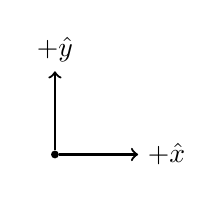
\begin{tikzpicture}
			\node[circle, fill, inner sep = 1pt] (origin) {};
			\node (y) [above = of origin] {$ +\hat{y} $};
			\node (x) [right = of origin] {$ +\hat{x} $};

			\foreach \node in {y, x}
				\draw[black, thick, ->] (origin) -- (\node);
		\end{tikzpicture}
		\begin{tikzpicture}
			\node (origin) { car };
			\node (left) [left = of origin] {$ f $};
			\node (above) [above = of origin] {$ N $};
			\node (below) [below = of origin] {$ m_\text{car}g $};

			\foreach \node in {left, above, below}
				\draw[black, thick, ->] (origin) -- (\node);
		\end{tikzpicture}
		\begin{align*}
			\sum F_y & = 0 \\
			N & = m_\text{car}g
		\end{align*}
		\begin{align*}
			W & = -fd \\
			W & = -\mu Nd \\
			W & = -\mu m_\text{car}gd
		\end{align*}
		\begin{align*}
			W & = E_f - E_i \\
			-\mu m_\text{car}gd & = 0 - \frac{1}{2}m_\text{car}v_i^2 \\
			d & = \frac{v_i^2}{2\mu g}
		\end{align*}
		\bc{ d = \frac{v_i^2}{2\mu g} }
	\item By what factor would the minimum stopping distance change if
		\begin{enumerate}[label = \textbf{(\roman*)}]
			\item \label{6.31.b.i} the coefficient of kinetic friction were doubled?
				\begin{align*}
					\mu & = 2\mu
				\end{align*}
				\begin{align*}
					W & = E_f - E_i \\
					-2\mu m_\text{car}gd_1 & = -\frac{1}{2}m_\text{car}v_i^2 \\
					d_1 & = \frac{v_i^2}{4\mu g}
				\end{align*}
				\begin{align*}
					d & : d_1 \\
					\frac{v_i^2}{2\mu g} & : \frac{v_i^2}{4\mu g} \\
					1 & : \frac{1}{2}
				\end{align*}
				\bc{\frac{1}{2}}
			\item \label{6.31.b.ii} the initial speed were doubled?
				\begin{align*}
					v_i & = 2v_i
				\end{align*}
				\begin{align*}
					W & = E_f - E_i \\
					-\mu m_\text{car}gd_1 & = -\frac{1}{2}m_\text{car}(2v_i)^2 \\
					d_1 & = \frac{2v_i^2}{\mu g}
				\end{align*}
				\begin{align*}
					d & : d_1 \\
					\frac{v_i^2}{2\mu g} & : \frac{2v_i^2}{\mu g} \\
					1 & : 4
				\end{align*}
				\bc{4}
			\item both the coefficient of kinetic friction and the initial speed were doubled? \\
				We can use parts \ref{6.31.b.i} and \ref{6.31.b.ii} to find the ratio as the $ W $ and $ E_f $ would simply expand to include the calculated values above and simplify to the expression below:
				\begin{align*}
					4 \cdot \frac{1}{2} & = 2
				\end{align*}
				\bc{2}
		\end{enumerate}
\end{enumerate}

\subsection{6.33}

\begin{align*}
	m_1 = m_2 = m_3 & = \SI{8.50}{\kilogram} \\
	k & = \SI{7.80}{\kilo \newton \per \meter} = \SI{7.80e3}{\newton \per \meter} \\
	x & = \SI{12.0}{\centi \meter}
\end{align*}

\begin{enumerate}[label = \textbf{(\alph*)}]
	\item Draw a free-body diagram of each mass. \\
		\begin{tikzpicture}
			\node[circle, fill, inner sep = 1pt] (origin) {};
			\node [below = of origin] (y) {$ +\hat{y} $};
			\node [right = of origin] (x) {$ +\hat{x} $};

			\foreach \node in {y, x}
				\draw[black, thick, ->] (origin) -- (\node);
		\end{tikzpicture}

		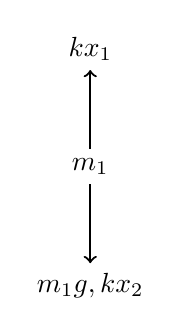
\begin{tikzpicture}
			\node (origin) {$ m_1 $};
			\node (above) [above = of origin] {$ kx_1 $};
			\node (below) [below = of origin] {$ m_1g, kx_2 $};

			\foreach \node in {above, below}
				\draw[black, thick, ->] (origin) -- (\node);
		\end{tikzpicture}
		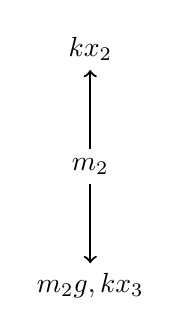
\begin{tikzpicture}
			\node (origin) {$ m_2 $};
			\node (above) [above = of origin] {$ kx_2 $};
			\node (below) [below = of origin] {$ m_2g, kx_3 $};

			\foreach \node in {above, below}
				\draw[black, thick, ->] (origin) -- (\node);
		\end{tikzpicture}
		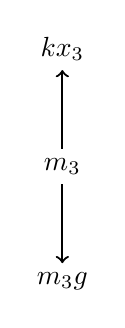
\begin{tikzpicture}
			\node (origin) {$ m_3 $};
			\node (above) [above = of origin] {$ kx_3 $};
			\node (below) [below = of origin] {$ m_3g $};

			\foreach \node in {above, below}
				\draw[black, thick, ->] (origin) -- (\node);
		\end{tikzpicture}
	\item How long is each spring when hanging as shown?
		\begin{align*}
			\sum F_y^{(m_3)} & = 0 \\
			kx_3 & = m_3g \\
			x_3 & = \frac{m_3g}{k} \\
			x_3 & = \frac{(\SI{8.50}{\kilogram})(\SI{10}{\meter \per \second \squared})}{\SI{7.80e3}{\newton \per \meter}} \\
			x_3 & = \SI{0.011}{\meter}
		\end{align*}
		\begin{align*}
			\sum F_y^{(m_2)} & = 0 \\
			kx_2 & = m_2g + kx_3 \\
			x_2 & = \frac{m_2g + kx_3}{k} \\
			x_2 & = \frac{(\SI{8.50}{\kilogram})(\SI{10}{\meter \per \second \squared}) + (\SI{7.80e3}{\newton \per \meter})(\SI{0.011}{\meter})}{\SI{7.80e3}{\newton \per \meter}} \\
			x_2 & = \SI{0.022}{\meter}
		\end{align*}
		\begin{align*}
			\sum F_y^{(m_1)} & = 0 \\
			kx_1 & = m_1g + kx_2 \\
			x_1 & = \frac{m_1g + kx_2}{k} \\
			x_1 & = \frac{(\SI{8.50}{\kilogram})(\SI{10}{\meter \per \second \squared}) + (\SI{7.80e3}{\newton \per \meter})(\SI{0.022}{\meter})}{\SI{7.80e3}{\newton \per \meter}} \\
			x_1 & = \SI{0.033}{\meter}
		\end{align*}
\end{enumerate}

\subsection{6.45}

\subsection{6.48}

\subsection{6.51}

\subsection{7.5}

\subsection{7.9}

\subsection{7.35}

\subsection{7.40}

\subsection{7.58}

\section{Lab Manual}

\subsection{871}

\subsection{876}

\subsection{884}

\subsection{885}

\end{document}
